\documentclass[10pt]{article}
\usepackage[polish]{babel}
\usepackage[utf8]{inputenc}
\usepackage[T1]{fontenc}
\usepackage{amsmath}
\usepackage{amsfonts}
\usepackage{amssymb}
\usepackage[version=4]{mhchem}
\usepackage{stmaryrd}
\usepackage{graphicx}
\usepackage[export]{adjustbox}
\graphicspath{ {./images/} }

\title{EGZAMIN WSTĘPNY Z MATEMATYKI }

\author{}
\date{}


\begin{document}
\maketitle
Egzamin składa się z 30 zadań. Zadania 1-10 oceniane będą w skali 0-2 punkty, zadania \(11-30\) w skali \(0-4\) punkty. Czas trwania egzaminu - 240 minut.

\section*{Powodzenia!}
\begin{enumerate}
  \item Rozwiązać nierówność \(2^{|x+1|} \leqslant 0,(9)\).
  \item Obliczyć resztę z dzielenia wielomianu \(w(x)=x^{101!}-x+1\) przez dwumian \(x+1\).
  \item Wyznaczyć dziedzinę funkcji \(f(x)=\log _{2} \log _{\frac{1}{2}} x^{2}\).
  \item Rozwiązać nierówność \(\cos (\pi-x) \leqslant \sin \left(\frac{\pi}{2}+x\right)\).
  \item Obliczyć największą wartość funkcji \(f(x)=\frac{1}{x^{2}+6 x+16}\).
  \item Dany jest ciąg \(\left(a_{n}\right)\), gdzie \(a_{n}=\frac{3-n}{n} \cos n \pi\) dla \(n \in N\). Zbadać monotoniczność ciągu \(\left(b_{n}\right)\), w którym \(b_{n}=a_{2 n-1}\) dla każdego \(n \in N\).
  \item Trzecim wyrazem ciągu arytmetycznego jest liczba 1. Obliczyć sumę pierwszych pięciu wyrazów tego ciągu.
  \item Wśród rozpoczynających studia wyższe jest tyle samo mężczyzn co kobiet. Co czwarta kobieta i co drugi mężczyzna z tych, którzy rozpoczęli studia, nie kończy ich. Obliczyć jaki procent liczby wszystkich absolwentów wyższych uczelni stanowi liczba absolwentek tychże uczelni.
  \item Rys. 1 przedstawia szkic wykresu funkcji \(y=f(x)\) dla \(x \in\langle 0 ; 4\rangle\). Określić dziedzinę i naszkicować wykres funkcji \(y=f(-x+3)\).
  \item Rozwiązać równanie \(x+\frac{x^{2}}{2}+\frac{x^{3}}{4}+\frac{x^{4}}{8}+\ldots=\frac{x+1}{3}\).\\
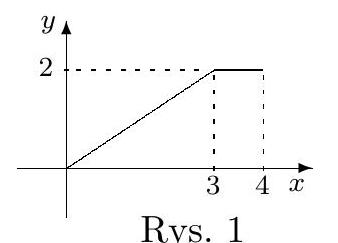
\includegraphics[max width=\textwidth, center]{2024_11_21_7f9effa233da5317fab2g-1}
\end{enumerate}

Rys. 1\\
11. Dla jakich wartości parametru \(a\) układ równań \(\left\{\begin{array}{l}x-a y=1 \\ a x-y=1\end{array}\right.\) ma co najmniej jedno rozwiązanie?\\
12. Przedsiębiorstwo proponuje dziesięcioletni kontrakt swojemu pracownikowi. W pierwszym roku pracy pracownik zarobi 15000 PLN, a w każdym następnym roku jego zarobki będą wzrastały o \(8 \%\). Ile zarobi pracownik w dziesiątym roku pracy? Ile wyniosą łączne zarobki pracownika za dziesięć lat pracy w przedsiębiorstwie? \(\left(\right.\) W obliczeniach można przyjaćc, że \(\left.(1,08)^{9}=2.\right)\)\\
13. Dla jakich wartości parametru \(m\) pierwiastki równania \(m x^{2}-2 m x+1=0\) spełniają nierówność \(x_{1}^{2}+x_{2}^{2}<3\) ?\\
14. Obliczyć pole obszaru opisanego układem nierówności \(\left\{\begin{array}{l}|x-1|-y \leqslant 0, \\ |x-2|+y \leqslant 3 .\end{array}\right.\)\\
15. Punkty \(A(2,1)\) i \(B(8,3)\) są wierzchołkami trójkąta \(A B C\). Wyznaczyć współrzędne wierzchołka \(C\), jeśli środkowe trójkąta \(A B C\) przecinaja się w punkcie \(M(4,5)\).\\
16. Obliczyć pole trójkąta wyznaczonego przez punkt \(A(3,2)\) i tę średnicę okręgu \(x^{2}-2 x+y^{2}+4 y=20\), która jest równoległa do prostej \(4 y-3 x=0\).\\
17. Dobrać parametr \(a\) tak, aby funkcja \(f(x)=\left\{\begin{array}{cl}\frac{\sqrt{1+x^{2}}-1}{x^{2}} & \text { dla } x \neq 0 \\ 2^{a} & \text { dla } x=0\end{array}\right.\) była ciągła.\\
18. Obliczyć \(\lim _{x \rightarrow 0^{+}} f^{\prime}(x)\), jeśli \(f(x)=\sin (\pi \cos \sqrt{x})\).\\
19. Rozwiązać równanie \(\cos 2 x+\cos x+1=0\) dla \(x \in\langle 0 ; 2 \pi\rangle\).\\
20. Rozwiązać nierówność \(x \sqrt{3-2 x}+1 \leqslant 0\).\\
21. Wyznaczyć liczby \(a\) i \(b\) takie, że \(\frac{1}{(x-1) x}=\frac{a}{x-1}+\frac{b}{x}\) dla \(x \in R-\{0,1\}\). Następnie obliczyć \(\lim _{n \rightarrow \infty}\left(\frac{1}{1 \cdot 2}+\frac{1}{2 \cdot 3}+\frac{1}{3 \cdot 4}+\ldots+\frac{1}{(n-1) n}\right)\).\\
22. Rys. 2 przedstawia kratę wymiaru \(4 \times 4\). Chcemy przejść po odcinkach tej kraty od punktu \(A\) do punktu \(B\) możliwie najkrótszą drogą. Ile jest takich dróg?\\
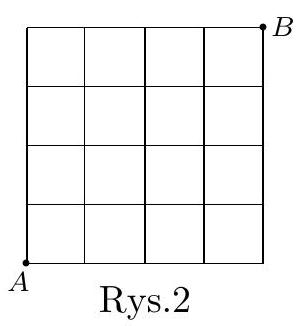
\includegraphics[max width=\textwidth, center]{2024_11_21_7f9effa233da5317fab2g-2}\\
23. Zdarzenia losowe \(A\) i \(B\) są niezależne i \(P(A \cap B)=\frac{1}{3}\) oraz \(P(A \cup B)=\frac{9}{10}\). Obliczyć \(P(A), P(B)\) i \(P(A-B)\), gdy \(P(A)>P(B)\).\\
24. Rzucono raz pięcioma kostkami do gry. Jakie jest prawdopodobieństwo tego, że na wszystkich kostkach wypadła taka sama liczba oczek lub na każdej z nich wypadła inna liczba oczek?\\
25. Napisać równanie stycznej do wykresu funkcji \(f(x)=x+\sqrt{2-x} \mathrm{w}\) jego punkcie przecięcia z osią \(O x\).\\
26. Rozwiazać równanie \(\log _{3}(3 x)+\log _{x}(3 x)=\log _{9}\left(\frac{1}{3}\right)\).\\
27. Rys. 3 przedstawia szkic wykresu wielomianu stopnia trzeciego. Wyznaczyć ten wielomian i wyznaczyć współrzędne punktu \(P\), w którym ma on minimum lokalne.\\
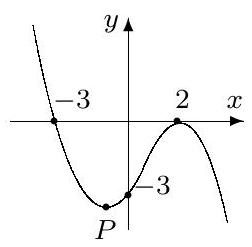
\includegraphics[max width=\textwidth, center]{2024_11_21_7f9effa233da5317fab2g-2(1)}

Rys. 3\\
28. Dane są punkty \(A(-1,3,3), B(0,1,5)\) i \(C(3,5,-1)\). Wyznaczyć taki punkt \(D\), że wektor \(\overrightarrow{A D}\) dzieli kąt między wektorami \(\overrightarrow{A B}\) i \(\overrightarrow{A C}\) na połowy i \(|\overrightarrow{A D}|=1\).\\
29. W równoramiennym trójkącie prostokątnym poprowadzono z wierzchołka kąta prostego dwie proste dzielące przeciwprostokątną na trzy odcinki jednakowej długości. Obliczyć cosinus kąta między tymi prostymi.\\
30. Oblilczyć objętość kuli stycznej do wszystkich krawędzi czworościanu foremnego o boku długości \(a\).


\end{document}